% Created 2021-04-13 Tue 20:05
% Intended LaTeX compiler: pdflatex
\documentclass[11pt]{article}
\usepackage[utf8]{inputenc}
\usepackage[T1]{fontenc}
\usepackage{graphicx}
\usepackage{grffile}
\usepackage{longtable}
\usepackage{wrapfig}
\usepackage{rotating}
\usepackage[normalem]{ulem}
\usepackage{amsmath}
\usepackage{textcomp}
\usepackage{amssymb}
\usepackage{capt-of}
\usepackage{hyperref}
\usepackage[a4paper, lmargin=30mm, rmargin=30mm, tmargin=25mm, bmargin=25mm]{geometry}
\usepackage{xurl}
\date{2021 April 13}
\title{TAB2XML Design Document\\\medskip
\large For version 1.0.0}
\hypersetup{
 pdfauthor={},
 pdftitle={TAB2XML Design Document},
 pdfkeywords={},
 pdfsubject={},
 pdfcreator={Emacs 27.1 (Org mode 9.4.4)}, 
 pdflang={English}}
\begin{document}

\maketitle
\tableofcontents

\newpage

\section{Introduction}
\label{sec:org7a5cdca}
TAB2XML is a system that can convert text tablature to MusicXML.  This document details the design of the system, in order to aid future developers of the system.  It describes both the high-level design of the system as a whole and the design of many individual components.
\section{System Design Overview}
\label{sec:org9bc5c92}
\begin{figure}[htbp]
\centering
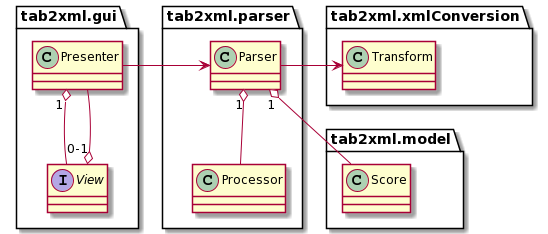
\includegraphics[width=.9\linewidth]{./Diagrams/full-system-diagram.png}
\caption{A diagram showing the relationship between major classes and packages.  Details about each component can be found in their respective section.  The arrows refer to classes that instantiate each other, but do not store instances as fields (i.e. they are instantiated and used within a method)}
\end{figure}

\subsection{Packages of TAB2XML}
\label{sec:orgeda408c}
TAB2XML is split into multiple packages.  The major ones are:
\begin{itemize}
\item tab2xml.exceptions - Stores TAB2XML's custom exception types
\item \hyperref[sec:org603a449]{tab2xml.gui} - Frontend and GUI related code
\item \hyperref[sec:org55b6b28]{tab2xml.model} - Abstraction of music
\item \hyperref[sec:org4f461cf]{tab2xml.parser} - Code that converts the tablature to a model representation
\item tab2xml.xmlconversion - Code that converts the model representation to MusicXML, and handles everything else XML related
\end{itemize}
There are also some more packages, but none have major classes.
\subsection{Major Classes of TAB2XML}
\label{sec:orga795dd7}
Here is a brief description of each class and interface in the above diagram.  Once again, full descriptions can be found in the classes's respective sections.
\begin{itemize}
\item \hyperref[sec:org7f1663d]{View} - Handles the GUI and interaction with the user
\item \hyperref[sec:org4d5aaed]{Presenter} - Handles interaction between the \texttt{View} and the backend code
\item \hyperref[sec:org4f461cf]{Parser} - Combines the components of the backend into a class that can fully transform a text tab to MusicXML
\item \hyperref[sec:org4d495dc]{Processor} - Pre-processes text tabs to make them easier to parse
\item \hyperref[sec:orge2b79c3]{Score} - A custom data structure that represents a parsed text tab
\item Transform - Transforms a \texttt{Score} into MusicXML
\end{itemize}
\newpage
\subsection{Converting Text Tabs}
\label{sec:orgc4020de}
\begin{figure}[htbp]
\centering
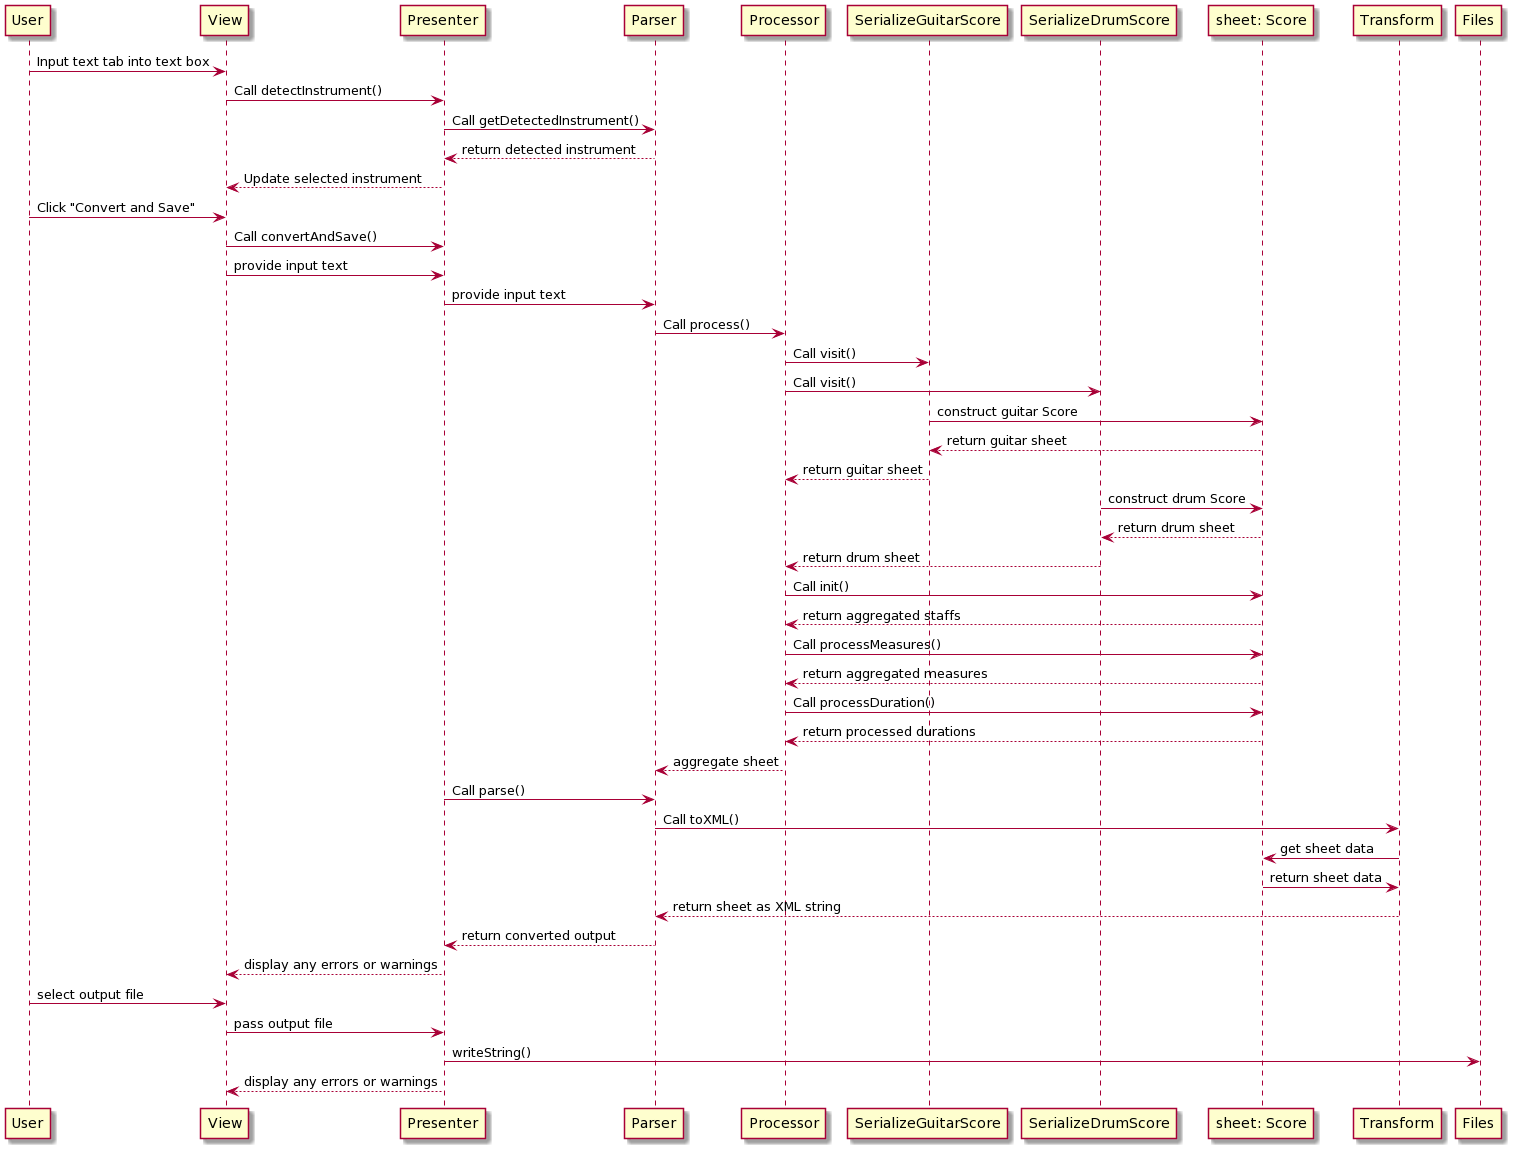
\includegraphics[width=.9\linewidth]{./Diagrams/convert-and-save-2.png}
\caption{A sequence diagram for the "Convert and Save" operation}
\end{figure}

Here is how the "Convert and Save" operation works:
\begin{enumerate}
\item The user inputs the tab into the input text box (by typing, copy-and-pasting, the "Load from File" button or dragging and dropping a file).
\item The \texttt{View} calls the backend method \texttt{Parser.getDetectedInstrument(String)} with its text as input.
\item If it succeeded, the \texttt{View} sets its selected instrument to the detected instrument.
\item The user inputs the necessary metadata into the \texttt{View}.
\item The user clicks the "Convert and Save" button.
\item The \texttt{View} calls the \texttt{Presenter}'s \texttt{convertAndSave()} method.
\item The \texttt{Presenter} calls the \texttt{View}'s \texttt{getInputText()} and \texttt{getSelectedInstrument()} methods to get the input tab and selected instrument.
\item The \texttt{Presenter} calls \texttt{View.getMetadata()} to get the metadata specified by teh user.
\item The \texttt{Presenter} creates a new instance of \texttt{Parser} with the obtained input text, instrument and metadata.
\item The \texttt{Parser} calls the \texttt{Processor} in order to process the input text tab.
\item In combination with the ANTLR code, a \texttt{Score} is constructed by \texttt{SerializeGuitarScore} and/or \texttt{SerializeDrumScore}.
\item The sheet is aggregated and returned to the \texttt{Parser}
\item The \texttt{Presenter} calls the \texttt{Parser}'s \texttt{parse()} method.
\item The \texttt{Parser} calls \texttt{Transform.toXML()}, which transforms the sheet data into a MusicXML string.
\item The \texttt{Parser} returns the MusicXML, as well as any errors that occurred.  Critical errors are thrown as Exceptions (which are caught and handled by the frontend), noncritical errors are returned.  This distinction exists so that critical errors stop the parsing, while noncritical errors do not stop it.
\item The \texttt{View} displays any errors or warnings to the user.
\item The \texttt{Presenter} calls the \texttt{View}'s \texttt{promptForFile} method to prompt the user for the desired destination file.
\item The \texttt{Presenter} calls \texttt{Files.writeString} to write the text tab to the selected file.
\item The \texttt{View} displays any errors that occurred during the file-saving operation.
\end{enumerate}
\newpage

\section{Front End Design}
\label{sec:org603a449}
\emph{All TAB2XML front-end code is located in the \texttt{tab2xml.gui} package.}
\subsection{Front End Classes}
\label{sec:orga8d6c4c}
\begin{figure}[htbp]
\centering
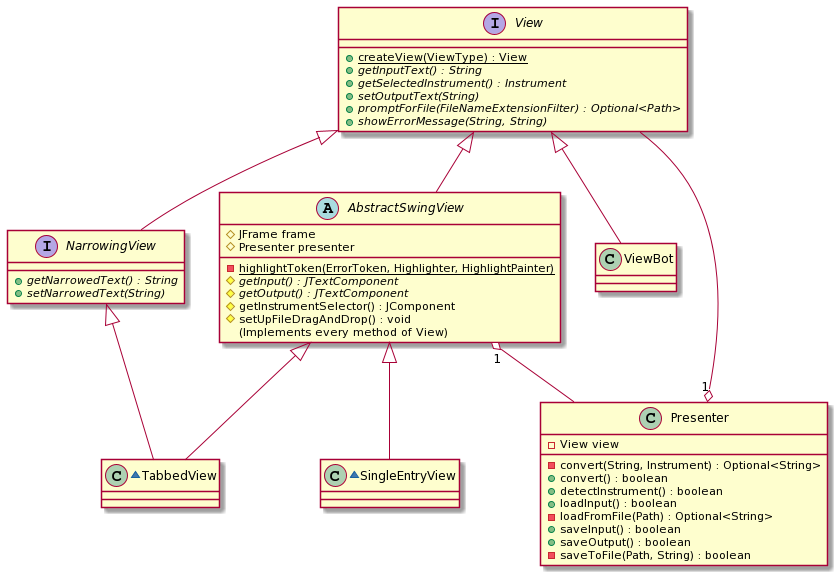
\includegraphics[width=.9\linewidth]{./Diagrams/frontend-class-diagram.png}
\caption{A class diagram for the frontend of TAB2XML.}
\end{figure}

The frontend of TAB2XML is designed using the \href{https://en.wikipedia.org/wiki/Model\%E2\%80\%93view\%E2\%80\%93presenter}{Model-View-Presenter (MVP)} paradigm.  It is divided into two main parts, the \texttt{View} and the \texttt{Presenter} (the Model is handled by the backend code).

The rationale behind this design is to reduce the effort involved in creating a new GUI.  If it extends \texttt{AbstractSwingView}, creating a new View is as simple as making a "mockup" Swing GUI and implementing two trivial methods.  This makes it easy to work with multiple GUIs at once (allowing the customer to choose which they prefer).  This design was especially important in the beginning of development, because the developers could prototype different GUI ideas with the customer using fully functional applications.  This system has enabled the TAB2XML development team to prototype three different GUIs so far, all of which are almost fully functional.
\subsubsection{The View}
\label{sec:org7f1663d}
The \texttt{View} is the part of the frontend that interacts with the user (the GUI).  It is handled by the \texttt{View} interface; all GUIs for TAB2XML implement the View interface.  In addition, all Views that represent a Swing GUI are subclasses of the skeletal implementation \texttt{AbsractSwingView}, which reduces the effort needed to make a View.

Currently, there are four concrete classes implementing \texttt{View}:
\begin{itemize}
\item \texttt{TabbedView} - The view currently in use, which supports all of TAB2XML's features.  It uses tabs to store the input and output separately.  The narrowing and metadata editing features are implemented in a sepearate class, the \texttt{EditingPanel}.
\item \texttt{SingleEntryView} - A view that uses a single text box for both input and output.  It was previously the default, but was superseded by \texttt{TabbedView} in version 0.3.0, and is currently unused.  It supports all of TAB2XML's features except measure narrowing and metadata editing.
\item \texttt{DoubleEntryView} - A view that uses two side-by-side text boxes for input and output.  It was only used early in development as a prototype, though extending \texttt{AbstractSwingView} means it supports the same features as \texttt{SingleEntryView}.
\item \texttt{ViewBot} - A class that simulates a GUI.  It is only used for testing.
\end{itemize}

The \texttt{NarrowingView} interface represents a \texttt{View} that supports TAB2XML's advanced measure-narrowing functionality.  Only \texttt{TabbedView} and \texttt{ViewBot} currently implement this interface.
\subsubsection{The Presenter}
\label{sec:org4d5aaed}
The \texttt{Presenter} is the part of the frontend that interacts with the backend code.  It is a single class, not an interface that has multiple implementations.  It implements behaviours such as converting a tab, loading from a file and detecting the instrument of the input tab.

It uses the View interface's public methods to interact with the view.  This means that the View's buttons can simply be linked to call the Presenter's methods, instead of having to implement the method in the View.  All of the Presenter's methods return either a \texttt{boolean} or an \texttt{Optional} to describe whether they succeeded or not, which is used by \texttt{TabbedView} to automatically switch tabs when a conversion operation succeeds.

The \texttt{Presenter} also handles interaction with files, though it does this by delegating to Java's \texttt{Files} class, simplifying the \texttt{Presenter} methods.
\subsection{Front End Maintenance}
\label{sec:orgf939879}
To create a new GUI, simply make your GUI handled by a class that extends \texttt{View}.  It should also have a \texttt{Presenter} field instantiated using \texttt{new Presenter(this)} (extending \texttt{AbstractSwingView} does this for you).  You must implement all of the \texttt{View}'s methods, which is much easier if you extend \texttt{AbstractSwingView}.

Once this is done, implementing functionality such as conversion is as simple as calling the appropriate method in \texttt{Presenter}.  Consult \texttt{Presenter}'s Javadoc documentation to determine which method to use.  For example, a Swing button called \texttt{convertButton} can be made to convert text tabs when pressed using the following code:
\begin{verbatim}
convertButton.addActionListener(e -> this.presenter.convert());
\end{verbatim}

To modify the look of an existing View such as \texttt{TabbedView} (or add/remove components), simply modify its constructor (you may have to edit the other methods, if they are broken by the change).  If you are adding a new feature that should exist in every Swing View, consider instead adding it to \texttt{AbstractSwingView}, as this will make it available for every View.

\newpage

\section{Back End Design}
\label{sec:org383671e}
\subsection{Overview}
\label{sec:orgb00dc15}
The backend of TAB2XML was designed with the main focus of flexibility, and future scaling of the system. The central component of the system is the \href{https://www.antlr.org/}{antlr4} parser generation tool. The system uses custom instrument defined grammar to recognize different formats of tablature. Since the system's grammar can be changed effortlessly this makes extending for different types of input much easier. With the combination of the generated antlr4 parser classes (located in \texttt{/src/generated/java}) and the system's custom model data classes, a tablature score can be abstracted into components which make handling the data simpler. The backend is divided into a three step process, the \texttt{preprocessing} of the tablature, the antlr4 \texttt{ParseTree} visitor which is used to extract score data, and finally the XML \texttt{conversion} process.

\subsection{Model Design}
\label{sec:org55b6b28}
\emph{All TAB2XML model code is located in the \texttt{tab2xml.model} package and its subsets \texttt{tab2xml.model.guitar} etc..}
\begin{figure}[htbp]
\centering
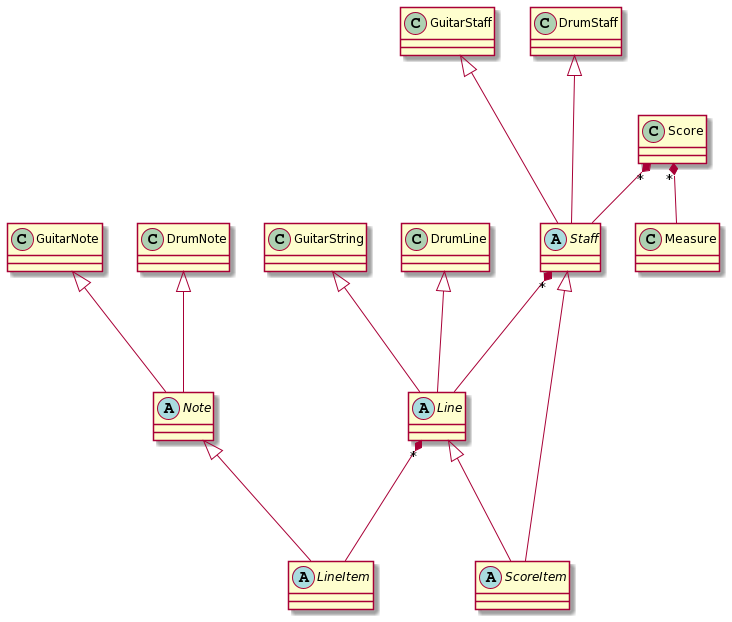
\includegraphics[width=.9\linewidth]{./Diagrams/backend-model-abstraction.png}
\caption{A general model diagram of the abstraction of a \texttt{Score} object.}
\end{figure}

The design of the instrument based model classes have a one-to-one correspondence between the respective grammar. The system abstracts some of these components which are shared in all the tablature formats (Such as \texttt{Score}, \texttt{Staff}, and \texttt{Note} objects). The \texttt{tab2xml.model} package contains general classes along with abstract data classes. In the model package, subsets \texttt{tab2xml.model.guitar} and \texttt{tab2xml.model.drum} are specific to the respective instruments. For example, a drum model will not contain a \texttt{Tune} representation and conversely a guitar model will not contain a \texttt{DrumType} representation.

\subsubsection{Score object}
\label{sec:orge2b79c3}
The \texttt{Score} object is by far the most important part of the model as it contains all the other objects. Because of this, the system is designed to allow the \texttt{Score} to be essentially a custom data structure. With functions such as adding staffs, iterating over staffs, iterating over notes and adding measures. One of the most important parts in designing this system for the \texttt{Score} object was to make sure that the notes had a natural ordering along with all other implementations of a \texttt{LineItem}. This would allow notes to be compared, sorted, and provide notes a positioning system. To achieve this, a custom iterator was defined along with the \texttt{Note} object being \texttt{Comparable}. This method of abstraction of the score has a lot of benefits during the tablature conversion process.
\begin{figure}[htbp]
\centering
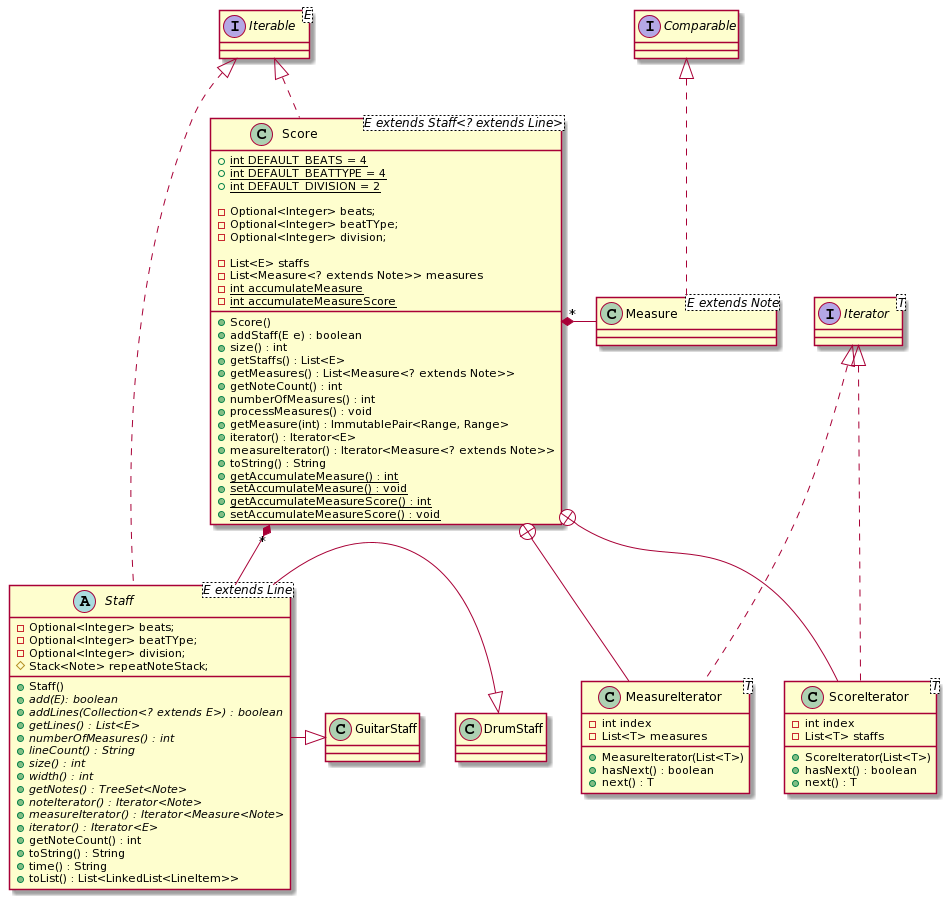
\includegraphics[width=.9\linewidth]{./Diagrams/backend-score-diagram.png}
\caption{A class diagram of a \texttt{Score} object.}
\end{figure}

\newpage
\subsection{Parser Design}
\label{sec:org4f461cf}
\begin{figure}[htbp]
\centering
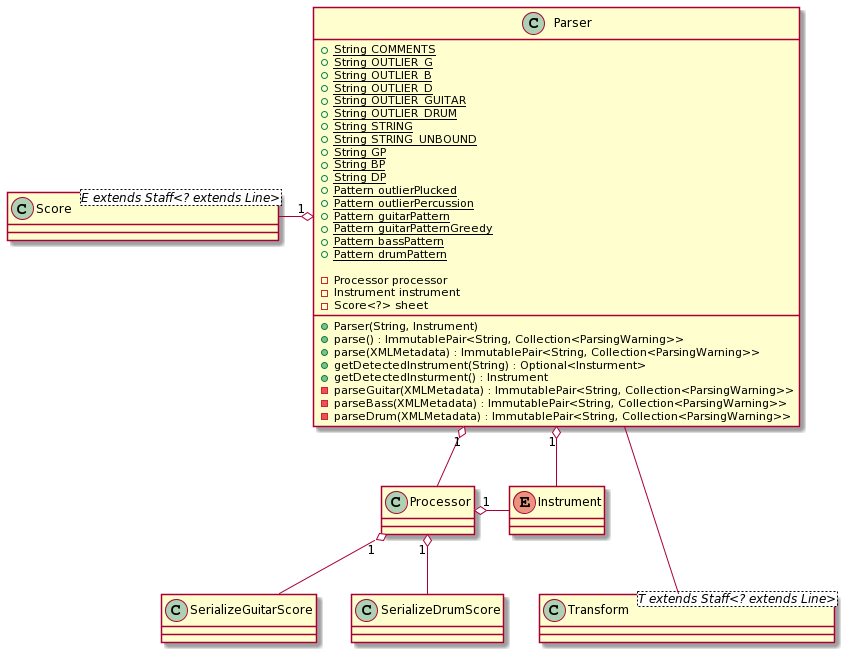
\includegraphics[width=.9\linewidth]{./Diagrams/backend-parser-class-diagram-p1.png}
\caption{A class diagram for the \texttt{Parser} class.}
\end{figure}

The highlighted areas in the figure below are the main components of the three main steps in the systems \texttt{Parser} process as mentioned earlier. The first is the \texttt{Processor} which is aggregated with the \texttt{Parser}. The responsibility of the \texttt{Parser} is to unite the \texttt{Processor} and the \texttt{Transform} components and delegate conversions of tablature based on selected instrument or detected instrument. The \texttt{Processor} preprocesses the input to prepare it for the \texttt{ParseTree} extraction process. One of its preprocess tasks is to comment the metadata around the detected staffs in the score (The grammars are defined to ignore the commented metadata, although we still extract it as it might be useful to the user). 
\begin{figure}[htbp]
\centering
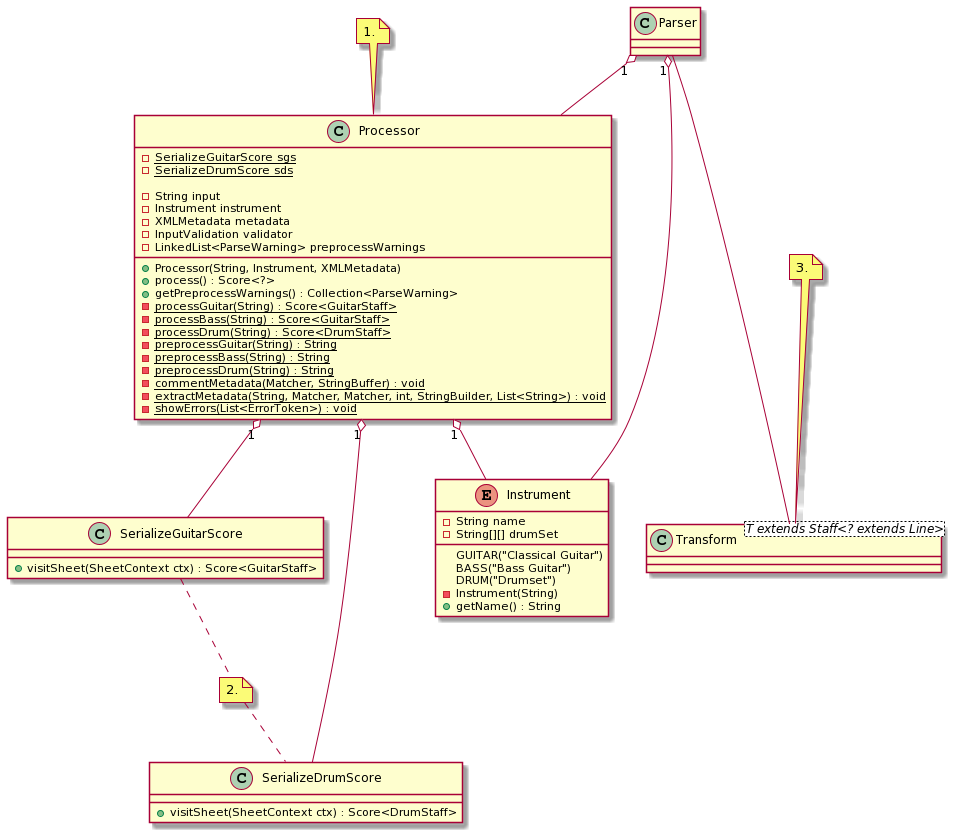
\includegraphics[width=.9\linewidth]{./Diagrams/backend-processor-diagram.png}
\caption{A class diagram for the \texttt{Processor} class and the 3 main stages.}
\end{figure}

\subsubsection{Sample Processor task}
\label{sec:org4d495dc}
before preprocessing:
\begin{verbatim}
	               III.......
	  |       |       |      :  |       |       |
E|--0-----------------------|-------------------------|
B|------------------3-----5-|-2-----------------------|
G|------------------3-------|-2-----------------------|
D|------------------5-------|-2-----------------------|
A|--------------------------|-0-----------------------|
D|--------------------------|-------------------------|
	                  3     4   1
\end{verbatim}

after preprocessing:
\begin{verbatim}
/*
	                 III.......
	  |       |       |      :  |       |       |
*/
E|--0-----------------------|-------------------------|
B|------------------3-----5-|-2-----------------------|
G|------------------3-------|-2-----------------------|
D|------------------5-------|-2-----------------------|
A|--------------------------|-0-----------------------|
D|--------------------------|-------------------------|
/*
	                  3     4   1
*/
\end{verbatim}

Once the main preprocessing tasks are complete and we are confident the input is valid, the \texttt{Processor} uses its aggregate extractor classes (ie. \texttt{SerializeGuitarScore}, \texttt{SerializeDrumScore}) to visit the parse tree generated by antlr4, while using the respective model classes to contain the information. The main steps of making the extracted data useful happens during the last steps of the \texttt{Processor}. Tasks such as creating measures for the \texttt{Score}, and calculating duration of notes. Once the processor has finished its job we have a \texttt{Score} object ready to be transformed into its XML equivalent. This is where The \texttt{Transform} class comes in. It's job is to simply generate XML from the parsed information serialized in the respective \texttt{Score} object. Hence, once this conversion is finished the XML is passed back to the frontend where it is handled as needed.

\newpage
\subsection{Grammar Design}
\label{sec:org07b7b69}
\begin{figure}[htbp]
\centering
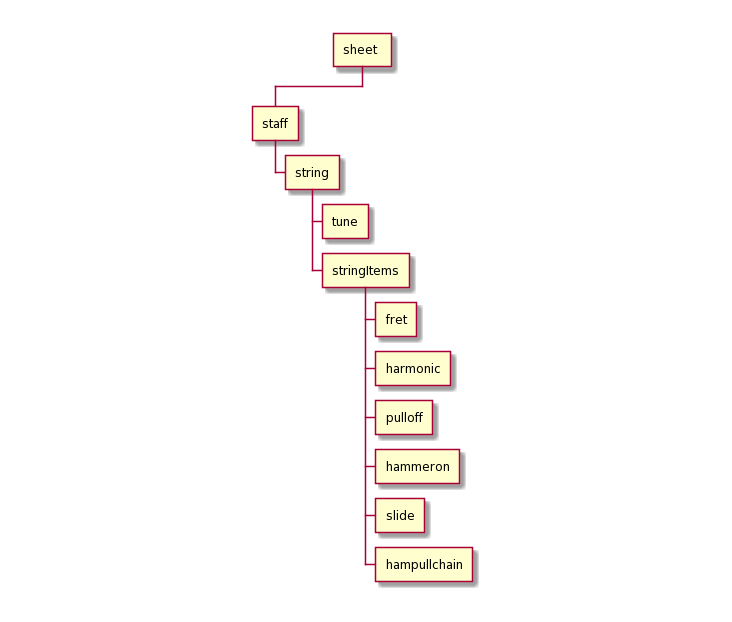
\includegraphics[width=.9\linewidth]{./Diagrams/backend-guitar-grammar-diagram.png}
\caption{An example of a basic \texttt{ParseTree} structure for a guitar(defined by \texttt{GuitarTab.g4} grammar):}
\end{figure}

The grammars for the system are designed to abstract the score representation. The grammars can be located at \texttt{src/main/antlr}. The system defines a set of rules for the grammar and antlr4 then creates a corresponding \texttt{ParseTree} from the input stream. The above are example rules (lower case, which would be nodes in the tree, sheet being the top level rule) built using different tokesn. This makes adding new support for tabs fairly easy as all you need to do is change the grammar rules and have a corresponding data model for that feature.

With the rules and \texttt{ParseTree} defined by antlr4, the system can traverse the \texttt{ParseTree} with the system’s custom made \texttt{Visitor} classes (\texttt{SerializeGuitarScore}, \texttt{SerializeDrumScore}). The visitors define their logic in parsing the information based on which node the visitor is at in the input stream. If a hammer-on rule is reached the information is stored in the respective \texttt{HammerOn} model class. The visitors are broken up into three abstract components that serializes the \texttt{Score}, serializes \texttt{Staff}, and finally collects line/string (\texttt{GuitarString}, \texttt{DrumLine}) items. These classes all extend  their respective grammar defined \texttt{BaseVisitor} classes generated by antlr4.

\subsection{XML-Related Design}
\label{sec:org2303c5d}
\subsubsection{The XMLMetadata Class}
\label{sec:org9632772}
The \texttt{XMLMetadata} class encodes all of the metadata a user can enter into the final score.  It contains a String variable for the tile, an Optional<String> for the composer (the reason why these are different is because the title has a default value while the composer does not), and a map mapping measure numbers to time signatures.  It can also return a map mapping measure \emph{ranges} to time signatures, which is used in the backend and computed by the \texttt{timeSignatureRanges()} method call then cached in the class.
\subsection{System capabilities}
\label{sec:org91aec1e}
The system can support well formed guitar and bass tablature very well. The system's auto instrument detection is robust as it takes into account the metadata around the main components of the score, making it convenient for the user.  The system does fall short when the input is not well formed due to a lacking input validation system which allows malformed input to bypass to the \texttt{ParseTree} visitor process. With the right implementation and design of a validation system this could be fixed rather easily. The grammars of this system could also be improved to further reduce ambiguities which arise errors. The system's design abstraction of the \texttt{Score} object into its subcomponents extends the possibility to allow more detailed configuration as desired by the user.

\subsection{Back End Maintenance}
\label{sec:org7f5ca75}
To add new support for a tablature feature you must change the grammar for the respective instrument. Adding a new rule is very simple but the main challenge is creating a grammar that avoids ambiguity. That’s why it’s important for the system to abstract the \texttt{Score} into subcomponents. For example, our system doesn’t support bend actions for guitar. We can add this support by adding a rule \texttt{bend} in our grammar file and finally add that rule to our \texttt{stringItems} rule. Then finally parsing the information once that rule is reached in the \texttt{ParseTree}. This ease of changing the grammar makes it easy to extend support. The grammars are not perfect but it is a good base to extend to more complex features. The model classes all contain modular abstractions of classes which make them easy to maintain or add additional changes to. There is a clear distinction of class separation since our model is divided based on the respective instrument. Making it simple to create new models for currently supported instruments or future instruments.

Sample Maintenance for Adding Bend notation:
\begin{enumerate}
\item Open \texttt{guitarTab.g4}.
\item Edit line 25 and add a rule \texttt{bend}.
\item Define the rule after the location the \texttt{hampullchain} rule is defined.
\item ie. \texttt{bend} : \texttt{fret'b'fret?} is a sample rule.
\item Add any data model classes as needed.
\item Add a corresponding \texttt{visit()} method in \texttt{ExtractStringItems.java} to collect the bend notes.
\item Update \texttt{GuitarTokens.java} located in \texttt{tab2xml.parser}.
\item Update \texttt{GuitarString.java} method, \texttt{getNotes()} to include the notes extracted from the new feature.
\end{enumerate}
\end{document}
